\onlyinsubfile{\setcounter{section}{4}}
\section{Extension: controlling for risk exposure}
\label{sec:exts}

% Reuse the Chapter 2 regression-table wrappers when this subfile is compiled on its own.
\providecommand{\ChapterTableNoteText}[1]{\parbox[t]{0.94\textwidth}{#1}}
\providecommand{\InputStataRegTable}[4]{%
\begin{table}[htbp]
\centering
\caption{#1}%
\label{#2}%
\begin{threeparttable}
\small
\begin{adjustbox}{max width=\textwidth}
\input{#3}%
\end{adjustbox}
\begin{tablenotes}[flushleft]
\footnotesize
\item \ChapterTableNoteText{#4}%
\end{tablenotes}
\end{threeparttable}
\end{table}%
}
\providecommand{\InputStataRegTableCompact}[4]{%
\begin{table}[htbp]
\centering
\caption{#1}%
\label{#2}%
\begin{threeparttable}
\begingroup
\footnotesize
\setlength{\tabcolsep}{4pt}%
\renewcommand{\arraystretch}{0.94}%
\begin{adjustbox}{max width=\textwidth}
\input{#3}%
\end{adjustbox}
\endgroup
\begin{tablenotes}[flushleft]
\footnotesize
\item \ChapterTableNoteText{#4}%
\end{tablenotes}
\end{threeparttable}
\end{table}%
}


\par The key point about the documented persistent component to returns is that, even when controlling for risk preferences and exposure, individuals systematic earn different returns on the same assets\footnote{This point is further corroborated by evidence of heterogeneity in returns on safe assets like deposit accounts. An example from the academic literature is \cite{Deuflhard14}, but one can compare rates offered on deposit account at commercial banks like Bank of America versus local banks and see similar discrepancies in everyday life.}. Moreover, the descriptive statistics for mean returns show that returns do not seem stable over the time period (ex.\ Global Financial Crisis). To address this concern, I re-estimate the cross-section (average returns) and panel (FE and CRE) specifications after augmenting the set of controls with portfolio-share variables (core assets, IRA assets, residential assets, long-term debt, and other debt) fully interacted with year dummies. 

\subsection{Trust and average returns}

\par I begin with the analysis of trust and average returns, now adding 2020 portfolio shares as an attempt at controlling for risk exposure by estimating the cross-sectional regression equation 

\[
\bar{r}^{net}_{i}
=
X_{i}'\beta
+ \sum_{j=1}^J \gamma_j s_{ji}
+ \varepsilon_{i}.
\]

\par Table~\ref{tab:41_avg_shares} shows that the hump-shaped relationship between trust and average returns survives this extension in both the baseline and extended specifications: the trust coefficients remain individually significant, and the joint test on the linear and quadratic trust terms is rejected in both columns.

\InputStataRegTableCompact{\textbf{Trust and Average Returns to Net Wealth with Portfolio-Share Controls}}{tab:41_avg_shares}{../../Code/Analysis/Tables/41_table1_avg_shares.tex}{OLS. Heteroskedasticity-robust standard errors. Trust and portfolio shares are measured in 2020; dependent variable is average returns to net wealth (winsorized). Column~\textit{(1)} uses the baseline controls from the main text plus asset and debt shares; column~\textit{(2)} adds the full demographic controls. For readability, footer rows for joint tests with $p \geq 0.10$ are omitted from the final presentation, though the underlying regressions include the full control set.}
\FloatBarrier

\par Relative to the corresponding average-return specifications in Table~\ref{tab:38_avg_returns}, adding shares increases model fit substantially: the adjusted $R^2$ in the baseline model rises from $.07$ to $.14$ and from $.09$ to $.17$ in the extended model. This suggests that portfolio composition explains a meaningful share of the cross-sectional variation in average returns. At the same time, the trust coefficients are essentially unchanged in sign and remain jointly significant, which is important for interpretation: controlling for observed portfolio shares improves fit, but it does not eliminate the hump-shaped relationship between trust and long-run returns. Furthermore, the Wald test on the coefficeints for the asset classes being jointly zero is rejected, suggesting that the proxies for risk exposure are predictive of returns to net wealth. 

\subsection{Augmenting the FE model}

\par I next add the portfolio-share controls to the panel regression model with respondent-level fixed effects. Since the FE model absorbs the time-invariant trust measure, the point here is not to estimate trust itself, but to see how much these proxies for risk exposure help explain within-respondent variation in returns.

\par Let  $j$ index asset classes.
\[
r^{net}_{it}
=
\alpha_i + \lambda_t + X_{it}'\beta
+ \sum_{j=1}^J
\left[
\gamma_j s_{jit}
+
\sum_{t' \in \mathcal{T} \setminus \{t_0\}} \delta_{jt'} \left( s_{jit} \cdot 1\{t = t'\} \right)
\right].
\]

\par Table~\ref{tab:41_fe_shares} shows the results of the estimation after adding the additional controls relevant to risk exposure. Relative to Table~\ref{tab:38_fe_1st}, adding the share controls increases the within-$R^2$ from $.18$ to $.20$ in both columns. The variance structure changes only modestly: $\rho$ falls from $.66$ and $.65$ to $.64$ and $.63$, while $\sigma_u$ stays around $.46$--$.47$ and $\sigma_e$ rises slightly from about $.33$ to $.35$. Thus, \textit{controlling for risk exposure does not effect the estimated distribution of fixed effects much.} This is useful information, since the indivdiual fixed effect is estimated after removing all time-varying variation from returns.

\InputStataRegTableCompact{\textbf{Panel OLS with Individual Fixed Effects and Portfolio-Share Controls}}{tab:41_fe_shares}{../../Code/Analysis/Tables/41_table2_fe_shares.tex}{Within (household) fixed-effects estimator. Standard errors clustered by household. Column~\textit{(1)} adds time-varying portfolio shares and share x year interactions to the baseline FE specification; column~\textit{(2)} adds the extended time-varying controls. Reported $\rho$, $\sigma_u$, and $\sigma_e$ are variance-component estimates from the FE decomposition. In the final table presentation, joint-test rows with $p \geq 0.10$ are omitted for readability, but all share and interaction terms remain in the regression.}
\FloatBarrier 

\par The joint tests on the remaining control variables also show a robustness to the risk controls. Age, wealth, and year effects remain strongly significant. The asset-share levels are not jointly significant, but the debt-share block is. Over time, the interaction terms for core shares, IRA shares, residential shares, and other debt are jointly significant, while the interaction for long-term debt is not. 

\subsubsection{Augmenting the CRE model}

\par The correlated random effects specification is the key panel model of interest here, since it retains the time-invariant trust measure while still allowing the persistent component to be correlated with the observed time-varying regressors.

\InputStataRegTableCompact{\textbf{The CRE (Mundlak) Model with Portfolio-Share Controls}}{tab:41_cre_shares}{../../Code/Analysis/Tables/41_table3_cre_shares.tex}{Random effects with respondent-level Mundlak means of the time-varying regressors, augmented with portfolio-share levels and share x year interactions. Standard errors clustered by household. Column~\textit{(1)} uses the baseline time-invariant controls; column~\textit{(2)} adds the full demographic controls. Reported $\rho$, $\sigma_u$, and $\sigma_e$ are variance-component estimates from the augmented CRE specification. ``Mundlak test $p$'' reports the cluster-robust Wald test of the null that the coefficients on all added panel means are jointly zero, the manual equivalent of Stata 19's \texttt{estat mundlak}.}
\FloatBarrier

\par The trust results survive this extension. The coefficients on trust remain positive on the linear term and negative on the quadratic term, and the joint test on the trust terms is still rejected in both columns. The corresponding Mundlak specification test is again overwhelmingly rejected, with $p \approx 3.7\times 10^{-43}$ in the baseline share-augmented CRE and $p \approx 7.0\times 10^{-43}$ in the extended specification, so the evidence against standard RE remains just as strong once portfolio composition is introduced. Relative to Table~\ref{tab:38_cre}, adding shares raises the within-$R^2$ from $.15$ to $.19$ in both columns. At the same time, $\rho$ falls from $.16$ and $.15$ to $.11$, which suggest a smaller share of the total variance is attributed to the persistent component after controlling for risk. Furthermore, $\sigma_u$ declines from about $.15$--$.16$ to $.12$, which implies that less unexplained variation is being attributed to persistent respondent-level differences. In other words, some of the previous variation across respondents has now been explained by risk exposure. Lastly, $\sigma_e$ remains around $.35$--$.36$.

\par The joint tests again show that the interaction structure does most of the work. The debt-share block is jointly significant, while the asset-share levels are not. But the interactions for core shares, IRA shares, residential shares, long-term debt, and other debt are all jointly significant. By contrast, the broader time-invariant blocks for education, race, and census region are not.

\par The key takeaway is that \textit{controlling for risk exposure in the CRE model increases explained variability, while retaining the hump-shaped relationship between trust and returns. The estiamted persistent component is estimated more accurately in terms of a smaller stndard deviation across respondents and a lower share of the total variance attributed to the persistent component.}

\subsection{Maximizing returns with trust}

\par As in the main text, I summarize the implied interior turning point of the quadratic trust specification by reporting the trust level that maximizes fitted returns. Because the FE model absorbs the time-invariant trust measure, the relevant comparison here is between the average-return model and the CRE model. Table~\ref{tab:41_trust_star_shares} shows that the turning-point calculations remain economically reasonable and statistically well determined in both baseline and extended specifications.

\InputStataRegTableCompact{\textbf{The Level of Trust which Maximizes Returns with Portfolio-Share Controls}}{tab:41_trust_star_shares}{../../Code/Analysis/Tables/41_table4_trust_star_shares.tex}{Trust$^*$ is computed as $-\hat\beta_1/(2\hat\beta_2)$ from the share-augmented quadratic specifications. Standard errors, $p$-values for $H_0\!:\mathrm{Trust}^*=0$, and 95\% confidence intervals use the delta method. ``Both sig?'' indicates whether the linear and quadratic trust terms are each significant at 10\%, while ``Joint test'' reports the Wald test on the two trust terms.}
\FloatBarrier

\par The estimated trust-maximizing values remain in the same moderate range emphasized in the main results. In the average-return regressions, the turning point lies around $6.3$ in the baseline specification and $6.7$ in the extended one; in the CRE regressions, it lies around $6.3$ and $6.6$. Compared with Table~\ref{tab:38_trust_star}, these values move only modestly once portfolio shares are added, with the CRE turning point especially stable. The confidence intervals remain fairly tight, and all reported turning points are statistically different from zero. Substantively, this reinforces the main conclusion: even after conditioning on detailed portfolio composition and its time-varying association with returns, the fitted relationship still suggests that households with moderate trust levels earn the highest returns to net wealth.

\subsection{The estimated distribution of fixed effects}

\par A final, but important comparison, is to take a look at the distribution of estimated fixed effects from the FE and CRE models with the full set of control variables extended to control for risk exposure. Figure ~\ref{fig:41_fe_cre_hist_shares} shows the final estimates of this persistent component of returns to net wealth across respondents in the survey. Interestingly, the estimated distribution from the CRE model seems to be less skewed than other empirical estimates suggest.

\begin{figure}[htbp]
\centering
\begin{minipage}[t]{0.48\textwidth}
\centering
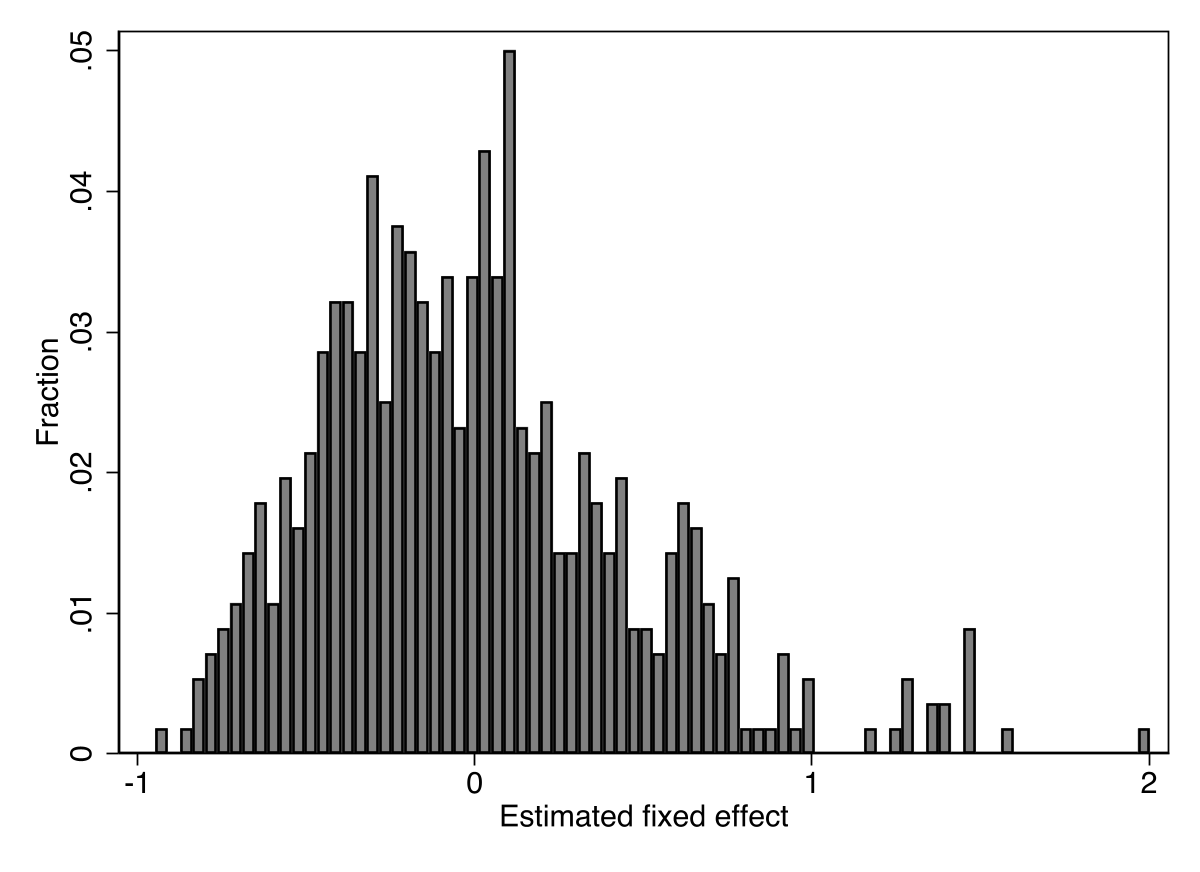
\includegraphics[width=\textwidth]{../../Code/Analysis/Figures/41_fe_hist_ext.png}
\end{minipage}\hfill
\begin{minipage}[t]{0.48\textwidth}
\centering
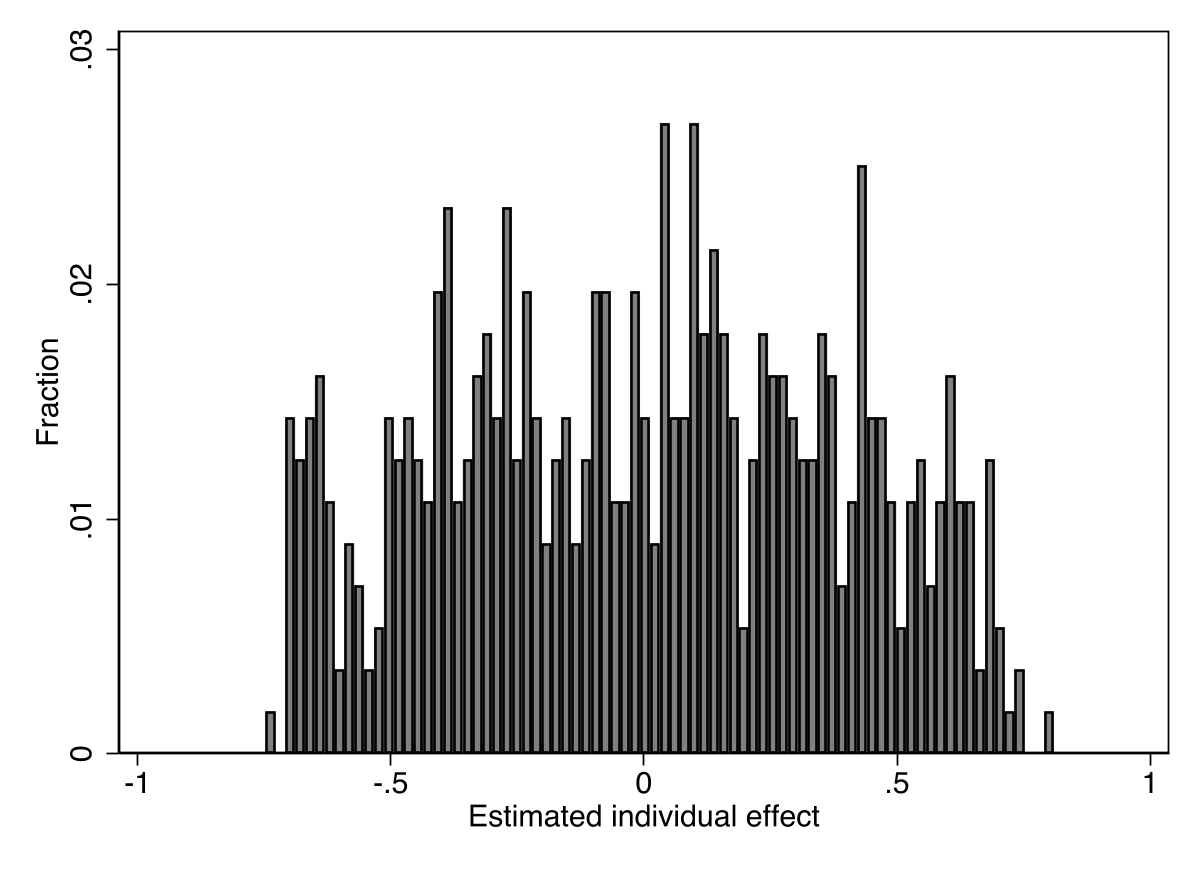
\includegraphics[width=\textwidth]{../../Code/Analysis/Figures/41_cre_hist_ext.png}
\end{minipage}
\caption{Distributions of estimated FE (left) and CRE (right) effects with portfolio-share controls included.}
\label{fig:41_fe_cre_hist_shares}
\end{figure}
\FloatBarrier

\begin{figure}[htbp]
\centering
\begin{minipage}[t]{0.48\textwidth}
\centering
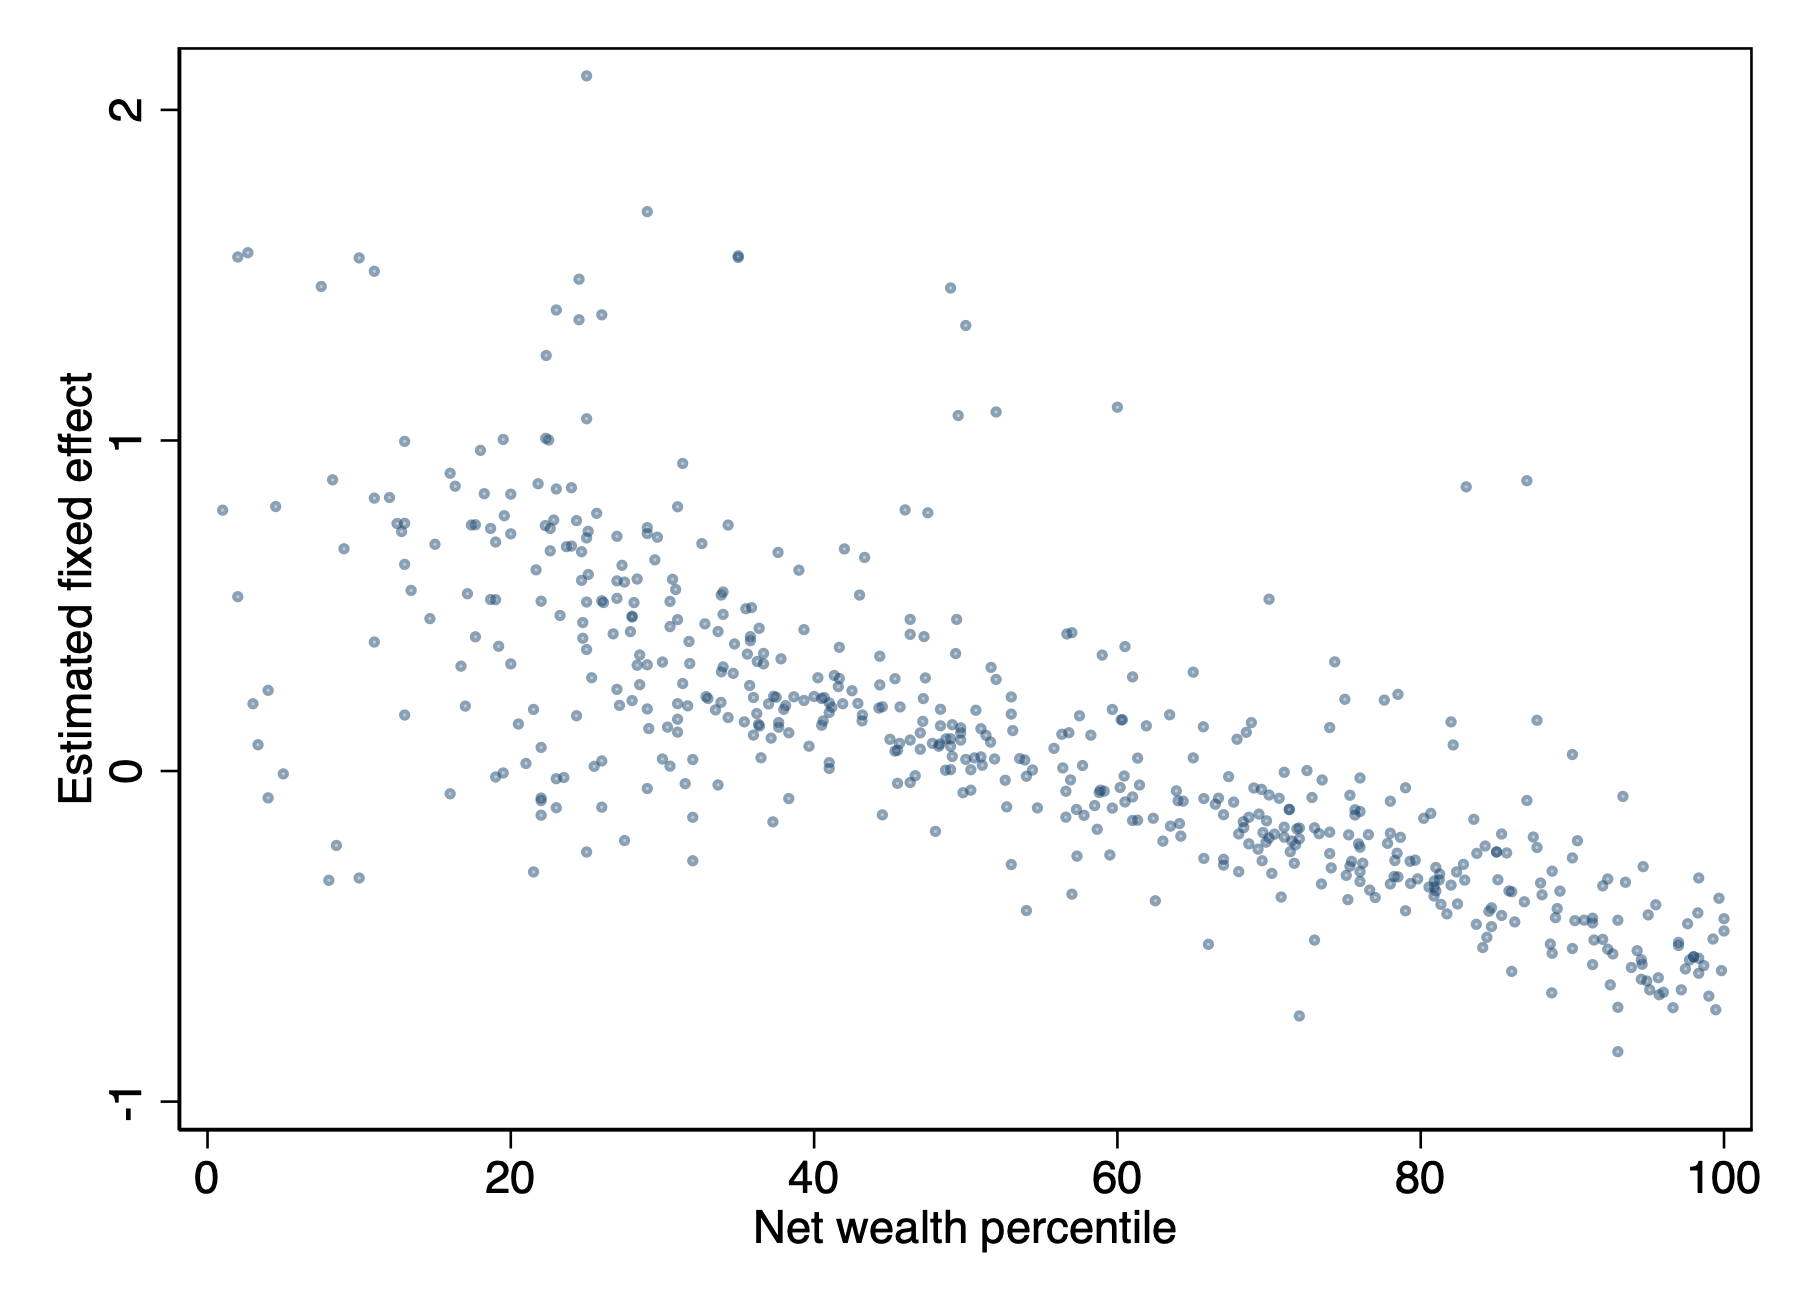
\includegraphics[width=\textwidth]{../../Code/Analysis/Figures/43_fe_vs_wpct_41ext.png}
\end{minipage}\hfill
\begin{minipage}[t]{0.48\textwidth}
\centering
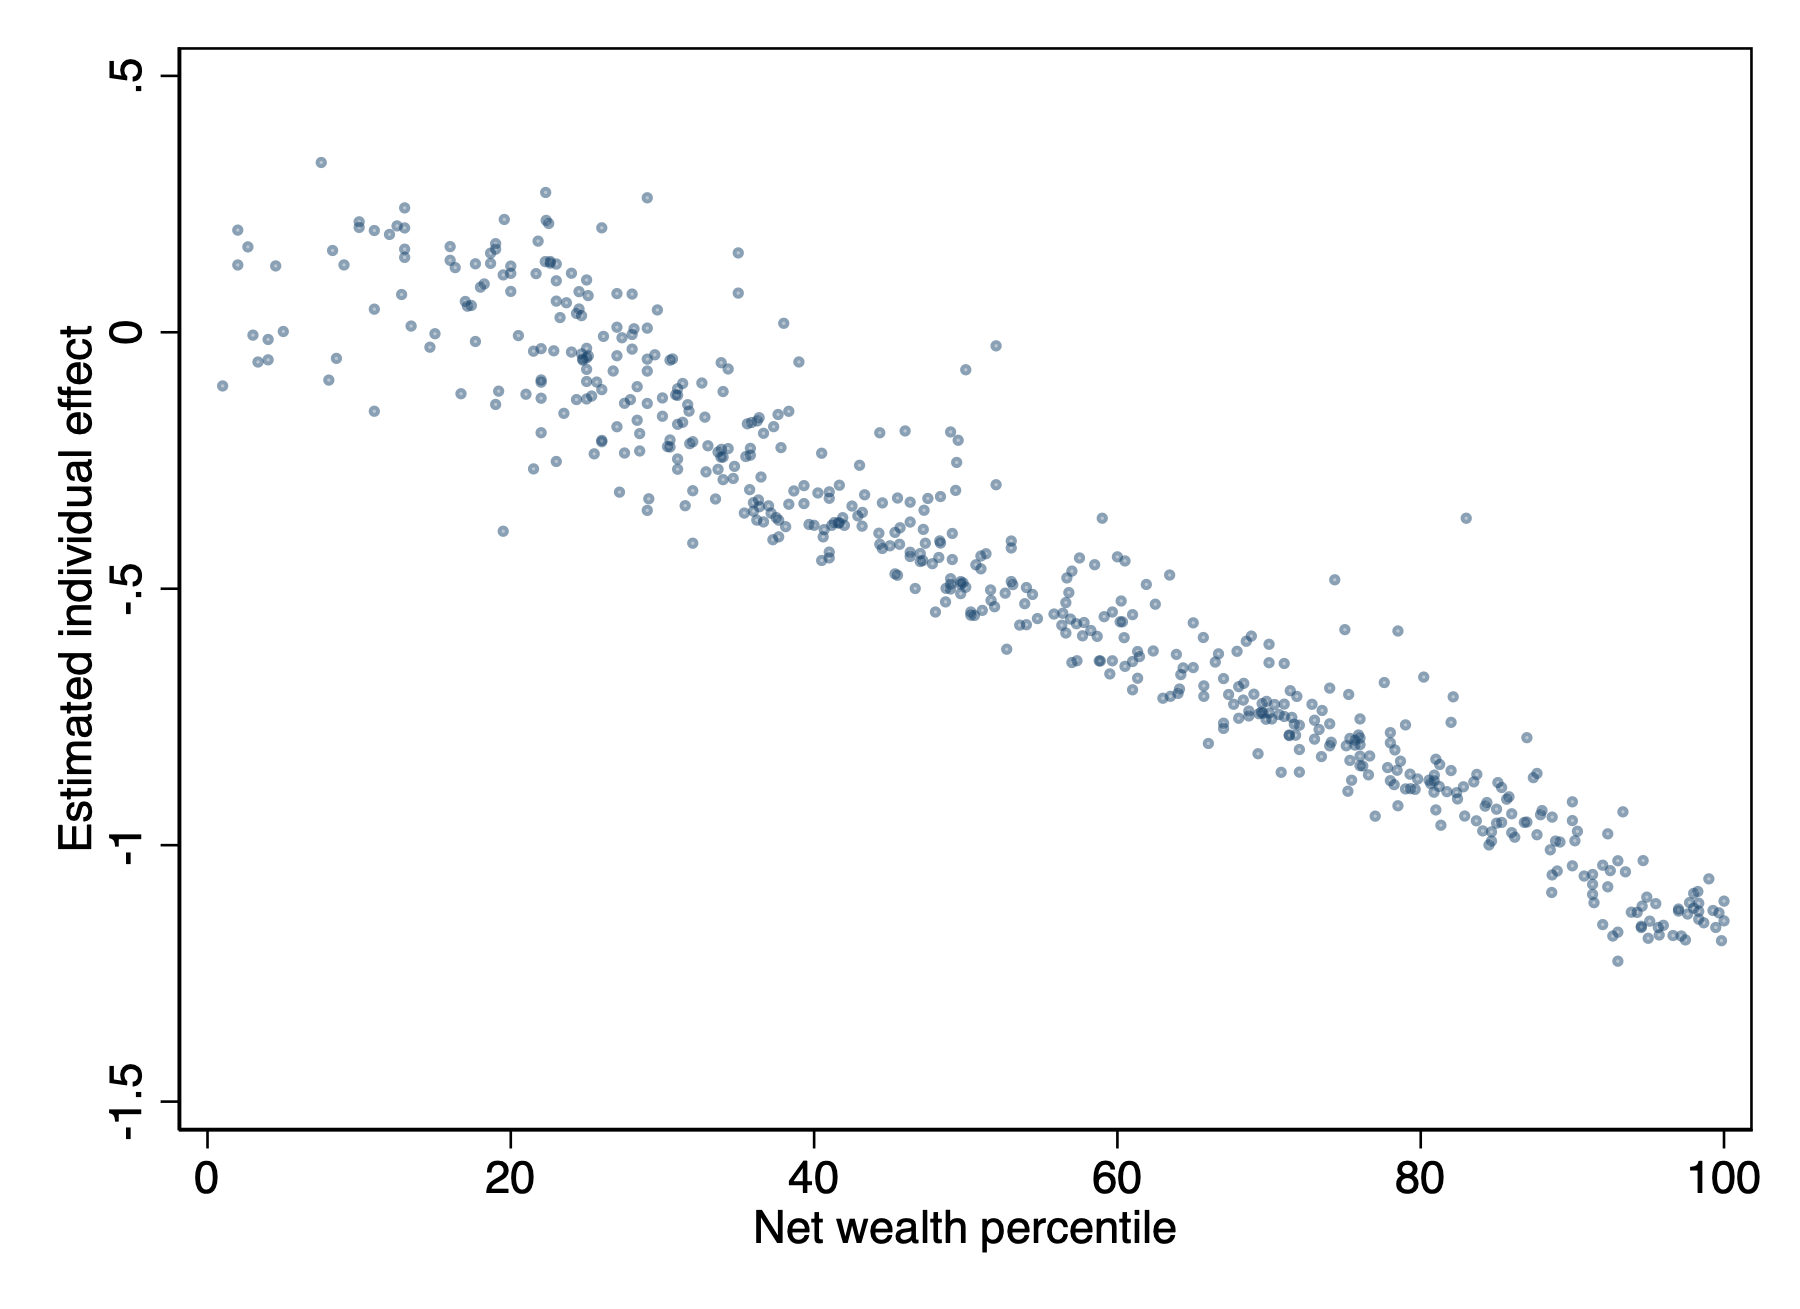
\includegraphics[width=\textwidth]{../../Code/Analysis/Figures/43_cre_vs_wpct_41ext.png}
\end{minipage}
\caption{Estimated FE (left) and CRE (right) individual effects vs.\ net wealth percentile, with portfolio-share controls.}
\label{fig:43_fe_cre_vs_wpct_shares}
\end{figure}
\FloatBarrier

\par Figure~\ref{fig:43_fe_cre_vs_wpct_shares} shows the same qualitative pattern after controlling for portfolio shares. In both the FE and CRE versions, the estimated individual effect remains downward sloping in wealth percentile. As in the main results, this should be interpreted as a feature of the residual persistent component after partialling out time-varying covariates and the share-by-year controls, not as a statement about the raw relationship between returns and wealth.
